\chapter{Work Performed}
\label{chap:Traballo Realizado}

\lettrine{T}{his} chapter presents the work carried out to adapt the IDIR framework to 2D retinal image registration. It begins with an overview of the process and a detailed description of the original IDIR method, followed by an explanation of the modifications made to adapt the system to the specific characteristics of fundus images. Subsequently, the datasets used, the experimental design developed, and the evaluation methods used to validate the results are described.

\section{Overview}
\label{sec:VistaXeral}

The work focused on adapting the IDIR framework, originally designed for thoracic 4D-CT, to the specific problem of 2D fundus image registration. This task required modifying the neural network architecture to operate in two dimensions, reformulating the regularization terms, and adapting the training and evaluation processes for the new domain.
To optimize the model, a systematic experimentation process was designed and specific training methodologies were developed. These include the creation of sampling strategies that prioritize regions of anatomical interest and techniques such as dynamic hyperparameter adjustment to refine model convergence.

Finally, to validate the results, an evaluation framework was built and applied to the FIRE dataset (which contains pairs of real images with different degrees of overlap and anatomical variations) and RFMiD (generated linear transformations), allowing assessment of different network characteristics. The evaluation combined objective quantitative metrics and qualitative visual analysis to ensure the quality and realism of the obtained deformations.

\section{IDIR}
\label{sec:IDIR}

IDIR (Implicit Deformable Image Registration) is a neural network-based image alignment method.
Its main difference compared to a traditional convolutional network is that,

What is proposed is to directly optimize the DFV using an implicit representation, so that the deformation is represented in the weights of an MLP themselves \cite{wolterink2021implicit}.

Other works like NIR \cite{sun2024medicalimageregistrationneural} or NODEO \cite{nodeo} propose similar registration methods that also use implicit representations of deformations, applied to brain magnetic resonance imaging.

\subsection{Architecture}
\label{subsubsec:Arquitectura}

A 3-layer MLP is used, and they experimentally determined that they obtained better results with 256 units per layer than 128.
For each training epoch (2500 in total), 10000 points are randomly sampled from the coordinate space within the mask.
The loss term is the normalized cross-correlation between the pixel values sampled in the fixed image and the corresponding ones in the moving image.
They use Adam as optimizer, with a learning rate of 0.0001.

[Continued translation follows same pattern - would you like me to continue with the rest?]\label{subsubsec:Termos de Perda}

The loss term is the function that is optimized during training, and it guides the network towards an optimal solution.
It quantifies the discrepancy between the network output and the desired result.

For the image registration task, two main categories of metrics are used to evaluate the alignment between images:
error-based metrics and similarity-based metrics. Error-based metrics (MSE, L1...) measure pixel-by-pixel differences between images,
being more sensitive to local differences and providing an absolute measure.
Similarity-based metrics (NCC, SSIM...) take into account structural patterns and statistical relationships between images, being more robust against variations in illumination and small displacements.
\cite{simmetric}

The main loss terms evaluated for this work are:

\begin{itemize}
    % Error-based metrics
    \item \textbf{MSE (Mean Squared Error)}:
    Average squared error between the fixed and moving image. It is sensitive to outliers and noise.
    \[
    \text{MSE} = \mathbb{E}[(Y - \hat{Y})^2] = \frac{1}{N} \sum_{i=1}^{N} (y_i - \hat{y}_i)^2
    \]
    where \( y_i \) is the pixel value of the fixed image, \( \hat{y}_i \) is the pixel value of the moving image, and \( N \) is the total number of pixels. \cite{Palubinskas02012017}

    Hyperelastic Regularizer in 2D   \item \textbf{L1 (Mean Absolute Error)}:
    Measures the average absolute error. Less sensitive to outliers than MSE.
    \[
    \text{L1} = \mathbb{E}[|Y - \hat{Y}|] = \frac{1}{N} \sum_{i=1}^{N} |y_i - \hat{y}_i|
    \]

    % Robust error metrics
    \item \textbf{Huber Loss}:
    Combines MSE and L1, being quadratic for small errors and linear for large errors.
    \[
    \text{Huber}(y, \hat{y}) = \begin{cases}
    \frac{1}{2}(y - \hat{y})^2 & \text{if } |y - \hat{y}| \leq \delta \\
    \delta(|y - \hat{y}| - \frac{1}{2}\delta) & \text{otherwise}
    \end{cases}
    \]
    where \( \delta \) is a hyperparameter that defines the transition point between quadratic and linear behaviors.

    \item \textbf{Smooth L1 Loss}:
    Similar to Huber Loss, but with a smooth transition between quadratic and linear regions.
    \[
    \text{SmoothL1}(y, \hat{y}) = \begin{cases}
    \frac{1}{2}(y - \hat{y})^2 & \text{if } |y - \hat{y}| \leq 1 \\
    |y - \hat{y}| - \frac{1}{2} & \text{otherwise}
    \end{cases}
    \]

    % Similarity-based metrics
    \item \textbf{NCC (Normalized Cross-Correlation)}:
    Evaluates the similarity between the two images by normalizing their intensities. It is invariant to changes in illumination.
    \[
    \text{NCC} = \frac{\sum_{i=1}^{N} (y_i - \mu_y)(\hat{y}_i - \mu_{\hat{y}})}{\sqrt{\sum_{i=1}^{N} (y_i - \mu_y)^2 \sum_{i=1}^{N} (\hat{y}_i - \mu_{\hat{y}})^2}}
    \]
    where \( \mu_y \) and \( \mu_{\hat{y}} \) are the means of the fixed and moving images, respectively.

    \item \textbf{SSIM (Structural Similarity Index)}:
    Evaluates the structural similarity between the two images, considering luminance, contrast, and structure.
    \[
    \text{SSIM}(y, \hat{y}) = \frac{(2\mu_y\mu_{\hat{y}} + C_1)(2\sigma_{y\hat{y}} + C_2)}{(\mu_y^2 + \mu_{\hat{y}}^2 + C_1)(\sigma_y^2 + \sigma_{\hat{y}}^2 + C_2)}
    \]
    where \( \mu_y \), \( \mu_{\hat{y}} \) are the means, \( \sigma_y \), \( \sigma_{\hat{y}} \) are the standard deviations, \( \sigma_{y\hat{y}} \) is the covariance, and \( C_1 \), \( C_2 \) are constants to avoid divisions by zero. \cite{Palubinskas02012017}
\end{itemize}

Due to the nature of retinal images, where there may be differences in illumination and contrast between the fixed and moving images,
it seems more appropriate to use similarity-based metrics such as NCC or SSIM.

NCC implementation was used from https://github.com/BDdeVos/TorchIR/blob/main/torchir/metrics.py.

\subsubsection{Regularization terms}\label{subsubsec:Regularization terms}

Since deformable image registration is an ill-posed problem, it is common to use some type of regularization on the DVF to avoid unrealistic deformations. Registration methods based on convolutional neural networks (CNN) represent DVFs as samples on a voxel grid, and therefore, spatial gradients can only be approximated through finite difference schemes (approximating derivatives through numerical calculation of differences between adjacent values in the grid). This is a computationally very expensive and inefficient process, and it implies discretization errors and loss of precision.

Using implicit representations, all operations are differentiable, and gradients can be easily computed analytically instead of having to approximate them, using PyTorch's autodifferentiation library.

Using ReLU as activation function, the network is differentiable once, while using a periodic activation function (like SIREN), the network is differentiable as many times as needed. This way, we can calculate any number of regularization terms and include them in the network optimization.

Some examples of regularization terms that can be used are:
\begin{itemize}
    \item Jacobian regularizer:
    The Jacobian determinant of the transformation (det ∇Φ) at a location x is an indicator of local stretching or compression.
    A negative or very close to 0 Jacobian determinant indicates that folding is occurring and the transformation will not be invertible.
    The Jacobian matrix is the matrix containing all partial derivatives of the transformation function (calculated using gradients).
    The Jacobian regularization term penalizes Jacobian determinant values that deviate from 1,
    trying to preserve local areas and avoid extreme stretching or folding.

    \begin{figure}[tbp]
        \centering
        \[
        S^{jac}[\Phi] = \int_{\Omega} \left| 1 - \det \left( \nabla \Phi \right) \right| \, dx
        \]
        \caption{Jacobian Regularizer}
    \end{figure}

    Ω represents the domain or region of space over which the transformation Φ is defined.
    
    \item Hyperelastic regularizer
    Constraints can also be added to the DVF with this term proposed by \cite{HyperelasticRegularization}.
    It consists of three terms, a length term, an area term and a volume term with the aim of controlling variations in these aspects.
    The length term penalizes variation in the length of DVF vectors, with u being the displacement measure of a point in space.
    The cofactor matrix of the transformation's Jacobian matrix controls the area,
    The maximum function ensures that only expansions exceeding a certain limit are penalized
    The determinant of the Jacobian matrix controls volume,
    and both penalize growth and contraction equally.
    αl, αa and αν are hyperparameters that control the importance of each term.

    \begin{figure}[tbp]
        \centering
        \[
        S^{hyper}[\Phi] = \int_{\Omega} \left[ \frac{1}{2} \alpha_1 |\nabla u|^2 + \alpha_a \varphi_c (\text{cof} \nabla \Phi) + \alpha_\nu \psi(\det \nabla \Phi) \right] dx,
        \]
        \[
        \text{Convex functions:} \quad \varphi_c(C) = \sum_{i=1}^3 \max \left\{ \sum_{j=1}^3 C_{ji}^2 - 1, 0 \right\}^2 \quad \text{and} \quad \psi(v) = \frac{(v-1)^4}{v^2}.
        \]
        \caption{Hyperelastic Regularizer}
    \end{figure}


    \item Bending energy penalty
    Deformation smoothness can be imposed using this penalty proposed in \cite{bendingenergy}, which
    requires that the second derivatives of the DVF be small throughout the domain, which prevents abrupt and discontinuous deformations.
    This term cannot be used in a network that uses ReLU as activation function, since the second derivative of a ReLU is always equal to 0.

    \begin{figure}[tbp]
        \centering
        \[
        S^{bending}[\Phi] = \frac{1}{8} \int_{-1}^{1} \int_{-1}^{1} \int_{-1}^{1} \left[ \left( \frac{\partial^2 \Phi}{\partial x^2} \right)^2 + \left( \frac{\partial^2 \Phi}{\partial y^2} \right)^2 + \left( \frac{\partial^2 \Phi}{\partial z^2} \right)^2 \right.
        \]
        \[
        \left. + 2 \left( \frac{\partial^2 \Phi}{\partial x \partial y} \right)^2 + 2 \left( \frac{\partial^2 \Phi}{\partial x \partial z} \right)^2 + 2 \left( \frac{\partial^2 \Phi}{\partial y \partial z} \right)^2 \right] dx\,dy\,dz
        \]
        \caption{Bending Energy Regularizer}
    \end{figure}
    
\end{itemize}

For the implementation in this work, all these terms were modified to work with two-dimensional transformations instead of three,
replacing the 3-dimension gradient in the Jacobian with a two-dimensional one, eliminating partial derivatives in z in bending energy and the volume term in the hyperelastic term.

\begin{itemize}
    \item Jacobian regularizer:\\
    \[
    S^{jac}[\Phi] = \int_{\Omega} \left| 1 - \det \left( \nabla \Phi \right) \right| \, dx \, dy
    \]
    \item Hyperelastic regularizer:\\
    \[
    S^{hyper}[\Phi] = \int_{\Omega} \left[ \frac{1}{2} \alpha_1 |\nabla u|^2 + \alpha_a \varphi_c (\text{cof} \nabla \Phi) \right] dx \, dy,
    \]
    \[
    \varphi_c(C) = \sum_{i=1}^2 \max \left\{ \sum_{j=1}^2 C_{ji}^2 - 1, 0 \right\}^2
    \]
    \item Bending energy penalty:\\
    \[
    S^{bending}[\Phi] = \frac{1}{8} \int_{-1}^{1} \int_{-1}^{1} \left[ \left( \frac{\partial^2 \Phi}{\partial x^2} \right)^2 + \left( \frac{\partial^2 \Phi}{\partial y^2} \right)^2 + 2 \left( \frac{\partial^2 \Phi}{\partial x \partial y} \right)^2 \right] dx \, dy
    \]
\end{itemize}

Regularization also has a significant impact on computation time, as it requires multiple backpropagation passes per epoch to calculate the different penalty terms.
Without regularization, only 1 pass is made to calculate the gradient of the image similarity term.
With Jacobian regularization, in addition to the similarity term, two derivatives (one per dimension) are calculated to obtain the Jacobian, resulting in 3 passes per epoch.
Adding hyperelastic regularization (without volume term), an additional derivative is needed for the Jacobian matrix cofactor, making a total of 4 passes per epoch.
Finally, with bending energy penalty, second derivatives are needed, which implies 7 passes per epoch in total.
In the original IDIR work, they used up to 13 passes because they work in 3D.

If the regularization terms have too much influence on the loss term, the network will make very small transformations to avoid being penalized, which will result in insufficient transformation.
On the other hand, if the terms are too small, the network will make very large transformations, which results in an unrealistic and overfitted transformation. This is especially evident in the case of the SIREN activation function, which tends to overfit easily due to its bias towards high-frequency signals.
The optimal amount of regularization depends on the specific pair of images to be aligned, so we will try to determine what is best for a sample of images.

Furthermore, although the different regularization terms value different aspects, it should be noted that there is also overlap in some of the properties they value.
For example, the hyperelastic regularizer can be considered a more general term that indirectly includes Jacobian penalties (both penalize "folding") and transformation smoothness (as bending does but to a lesser degree).

\subsubsection{Learning rate and batch size}
\label{subsubsec:Learning rate and batch size}

The learning rate is an optimizer parameter (Adam in this case) that regulates the size of adjustments made to model parameters during each update iteration.
It determines the magnitude of change applied to minimize the loss function, affecting both convergence speed and learning process stability.
Too high a learning rate can cause the network to diverge, while too low a learning rate can result in slow convergence or getting stuck in local minima.

Due to the nature of the network, the batch size used has a direct relationship with the learning rate, so we will try to determine the optimal relationship between both.

One of the most common heuristics for relating learning rate and batch size is the linear scaling rule \cite{goyal2018accuratelargeminibatchsgd}.
The rule indicates that the optimal learning rate should scale linearly with the number of samples per batch.

One way to explain this is that since with larger batch sizes we have a better approximation of the real gradient, it is possible to use a higher learning rate without the network diverging. \cite{kexuefm}

The batch size in this network represents the number of coordinates randomly sampled from the coordinate space within the mask.

\subsection{Method}\label{subsubsec:Method}

Being the objective to find an optimal spatial transformation between the moving image and the fixed image,
it is necessary to obtain the deformation function Φ(x) = u(x) + x that maps each coordinate x in the moving image to a coordinate in the fixed image,
so that the coordinate x in the fixed image anatomically corresponds to the coordinate Φ(x) in the moving image.
This problem can be formulated as an optimization problem where $L_{data}$ is a similarity metric between the fixed ($F$) and moving ($M$) images, $L_{reg}$ is a regularization term on the transformation Φ, and α is a weighting term.
\begin{equation}
    \hat{\Phi} = \operatorname*{Arg\,min}_{\Phi} L_{data}(M \circ \Phi, F) + \alpha L_{reg}(\Phi)
\end{equation}

The main innovation introduced by IDIR\cite{wolterink2021implicit} is that the transformation Φ is implicitly represented in the neural network.

Compared to a traditional CNN, this network does not receive pixel intensity values as input,
but rather receives spatial (continuous) coordinates and returns a new coordinate.
Since the network weights define the transformation, these can be directly optimized
using a similarity metric as the loss function.

Parameterizing the deformation function as an \glossary{INR} within an \glossary{MLP} has several advantages for image registration.
First, the transformation representation is continuous and therefore independent of image resolution,
thanks to this the same model can be used for images of any size, unlike a traditional CNN
which has to be adapted for each resolution.

Second, doing it this way allows leveraging the capabilities of libraries like PyTorch to calculate the gradients of the transformation with respect to coordinates.
This allows obtaining more precise gradients than finite difference approximations
and allows taking advantage of a large amount of literature on efficient regularization in medical images.

Third, the activation function used in the network can be modified to adjust it to the particular needs of the image registration task.

The \gls{NTK} describes how a neural network model responds to changes in its parameters during training,
and depending on the activation function used, the NTK varies and the network can be more or less sensitive to certain deformations.

Finally, a new network will be trained for each pair of images, this being a fairly small network in comparison and dispensing with the need for large datasets for its training.

\subsection{Replication of results}
\label{subsec:Replication of results}

The results obtained by Wolterink et al. \cite{wolterink2021implicit} shown in table \ref{tab:comparison} were replicated.

\begin{table}[ht]
    \centering
    \caption{Replication of IDIR results}
    \begin{tabular}{c|c}
        Scan & {IDIR / Replication} \\
        1  & 0.76 (0.94) / 0.79 (0.92) \\
        2  & 0.76 (0.94) / 0.71 (0.89) \\
        3  & 0.94 (1.02) / 0.95 (1.01) \\
        4  & 1.32 (1.27) / 1.32 (1.22) \\
        5  & 1.23 (1.47) / 1.23 (1.46) \\
        6  & 1.09 (1.03) / 1.15 (1.04) \\
        7  & 1.12 (1.00) / 1.11 (0.99) \\
        8  & 1.21 (1.29) / 1.20 (1.28) \\
        9  & 1.22 (0.95) / 1.16 (0.99) \\
        10 & 1.01 (1.05) / 1.09 (1.05) \\
        Average & 1.07 / 1.07 (1.08) \\
    \end{tabular}
    \label{tab:comparison}
\end{table}

\section{Adaptation to 2D}
\label{sec:Adaptation to 2D}

To adapt the IDIR model to 2D, it is necessary to modify the network architecture to work with two-dimensional images.
The original IDIR architecture has a 3-dimensional input (x, y, z) and a 3-dimensional output (dx, dy, dz),
while our network has a 2-dimensional input (x, y) and a 2-dimensional output (dx, dy).

The input and output layers of the network were modified to accept two-dimensional coordinates (originally [3, 256, 256, 256, 3], now [2, 256, 256, 256, 2]).

It was necessary to modify the interpolation functions, which previously interpolated three-dimensional values and now interpolate two-dimensional values.

The regularization terms were also adapted to work with two-dimensional coordinates, as detailed in section \ref{subsubsec:Regularization terms}.

Finally, the evaluation process had to be implemented from scratch to adapt to the new image and reference data format.

\subsection{Registration Process}
\label{subsec:Registration Process}

The registration of each pair of images (fixed and moving) is treated as an independent optimization problem. For each pair, a new neural network is trained from scratch whose sole objective is to learn the specific deformation that aligns those two images.

First, an instance of the MLP is created with the 2D architecture and hyperparameters such as the activation function, loss metric and regularization terms to be applied are defined. The initialization of the network weights is a particularly relevant step.

Once the network is initialized, a coordinate tensor is generated that contains the location (x, y) of all pixels that are within the mask of the fixed image. This tensor represents the complete coordinate space over which the network will learn the deformation.

Next, the training loop begins, which is repeated for a predefined number of epochs. In each iteration within an epoch, the following process is performed:
\begin{itemize}
    \item \textbf{Coordinate Sampling:} Instead of processing the entire image at each step, a subset of points from the coordinate tensor equal to the batch size is selected. The sampling strategy is a critical component that was the subject of experimentation in this work.

    \item \textbf{Prediction and Transformation Application:} The sampled (x, y) coordinates are input to the network. The MLP acts as an implicit deformation function, returning a displacement vector (dx, dy) for each input coordinate.

    \item \textbf{Loss Calculation:} To quantify how well the deformation aligns the images, intensity values are compared at the selected points. For each original coordinate (x,y) in the fixed image, the corresponding intensity value in the moving image is obtained at the transformed coordinate (x + dx, y + dy). Since the latter is usually a non-integer position, interpolation is used to estimate its intensity value. The loss metric (NCC, SSIM, etc.) calculates the discrepancy between the set of fixed image intensities and those obtained from the transformed moving image.

    \item \textbf{Backpropagation and Update:} The penalty terms calculated from the regularizers are added to the similarity loss value. The resulting total loss value is used to calculate the gradients with respect to the network weights through backpropagation. Finally, the optimizer (Adam) uses these gradients to update the MLP weights, adjusting them slightly in the direction that minimizes the loss.
\end{itemize}

This cycle repeats until all epochs are completed. At the end of training, the optimized weights of the network encapsulate the continuous and specific deformation function for that pair of images.

It is crucial to emphasize that the task of retinal image registration differs substantially from that of lungs. For this reason, it is not possible to assume that the optimal hyperparameters from the original work are valid for this new domain, which justifies the extensive experimentation performed.

\section{Datasets}
\label{sec:Datasets}

\subsection{FIRE}
\label{subsec:FIRE}

It consists of 134 pairs of retinal images, with a size of 2912 × 2912 pixels and a \gls{FOV} of 45◦× 45◦.
They are classified into 3 categories according to the degree of overlap and the presence of anatomical differences: \textit{S}, \textit{P} and \textit{A}. \cite{FIRE}

\begin{figure}[tbp]
    \centering
    \setlength{\tabcolsep}{8pt} % Adjust column spacing
    \begin{tabular}{|c|c|c|c|}
        \hline
        \textbf{Category} & \textbf{Number of image pairs} & \textbf{Overlap (\%)} & \textbf{Visual Differences} \\
        \hline
        \textbf{\textit{\textsf{S}}} & 71 & > 75 & No \\
        \hline
        \textbf{\textit{\textsf{P}}} & 49 & < 75 & No \\
        \hline
        \textbf{\textit{\textsf{A}}} & 14 & > 75 & Yes \\
        \hline
    \end{tabular}
    \caption{Classification of image pairs into categories.}
    \label{tab:categorias}
\end{figure}
\FloatBarrier

It includes 10 reference points for each image, which are used for registration evaluation, as well as a mask for each image that indicates the location of pixels with color information.

\begin{figure}[tbp]
    \centering
    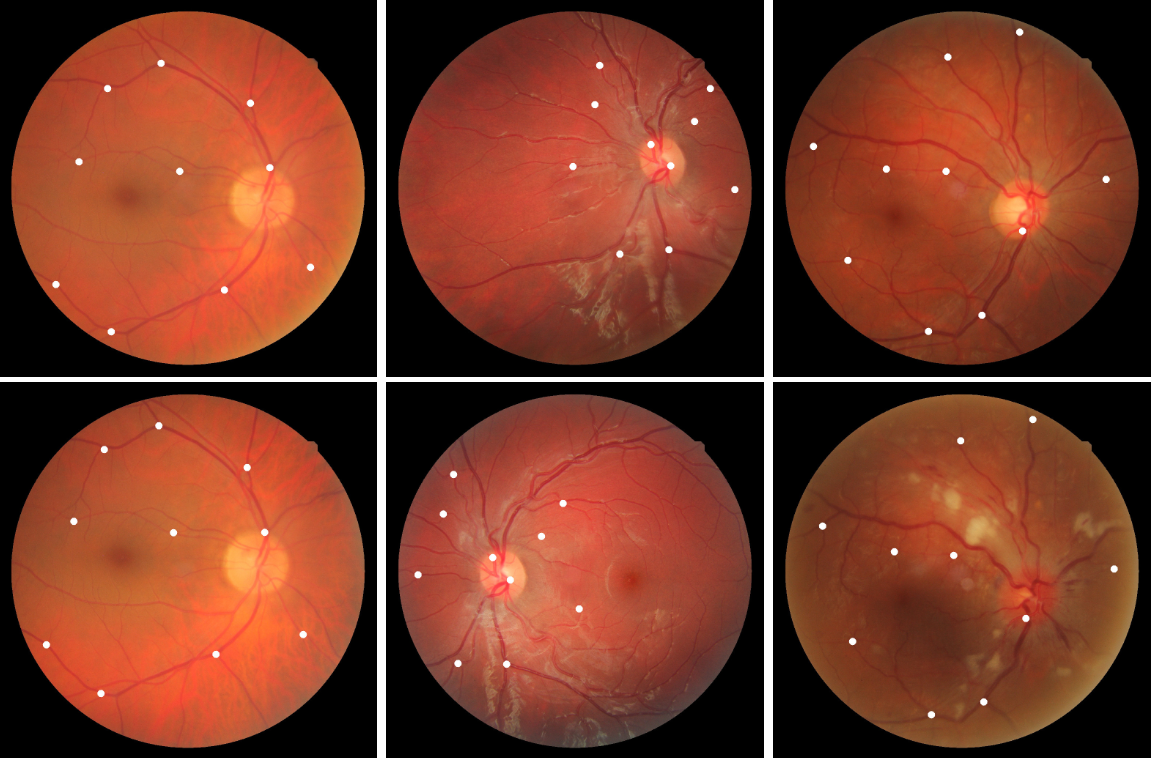
\includegraphics[width=0.8\textwidth]{imaxes/fire-ej.png}
    \caption{Example images from the FIRE dataset \cite{FIRE} with control points indicated. From left to right, categories \textit{\textsf{S}}, \textit{\textsf{P}}, \textit{\textsf{A}}.}
    \label{fig:fire_ej}
\end{figure}

\subsection{RFMID}\label{subsec:RFMID}

The RFMiD dataset \cite{RFMiD} provides 3200 color fundus images with 1712x1712 resolution, labeled according to whether they have any anomaly or not.
It also provides labels for 45 different anomalies annotated by experts.

To use it in this work, we selected a subsample and generated random transformations. We saved the original and transformed images as well as the associated transformation matrices for subsequent evaluation.
It is also divided between color and geometry transformations.

Figure \ref{fig:rfmid_ej} shows an example of an image pair from the RFMiD dataset.

\begin{figure}[tbp]
    \centering
    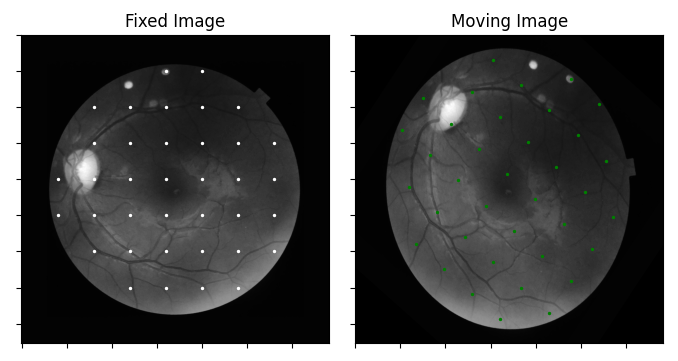
\includegraphics[width=0.8\textwidth]{imaxes/rfmid_ej.png}
    \caption{Example of images from the RFMiD dataset. The image on the left is fixed and the one on the right is moving.}
    \label{fig:rfmid_ej} 
\end{figure} 

\subsection{Differences between datasets}
\label{subsec:Diferencias entre os datasets}

An advantage of using two different datasets is that each has unique characteristics that allow evaluating the model in different contexts.
The main difference is that RMiFD is a synthetic dataset, in which we did not introduce color differences and they always have 100% overlap, so it only evaluates the model's ability to perform geometric registrations.
In contrast, FIRE is a real dataset, in which there are changes in illumination, contrast, overlap and other visual differences, so it evaluates the model's ability to perform registrations under much more adverse conditions.

\section{Experimental Design}
\label{sec:Diseño de Experimentos}

The experimental design is a systematic process that seeks to determine the influence of different factors on a specific outcome. In this case, the objective is to evaluate how different parameters affect the quality of image registration.

Computational cost is a very important factor to consider, since each combination of parameters requires a complete network training for each pair of images, which implies a high energy and time cost.
For example, to test a combination of parameters on FIRE, a network will have to be trained for each pair of images from the 134 in the dataset.
At a training time of 3 minutes per pair, complete training would take more than 6 hours for each parameter combination, with a memory footprint of around 5 GB of VRAM.
The temporal and memory cost depend on several factors, the most relevant being the regularization used, image resolution, batch size and activation function.
Specifically, SIREN has a much higher computational cost than ReLU, requiring about twice the time and memory to train the network.

Due to the large number of factors to consider, a phased experimentation approach was adopted.

Initial experiments were conducted to identify the most promising parameter ranges using a representative subsample of 14 image pairs from each FIRE dataset category, with the objective: Reduce the parameter space for subsequent phases.
In this phase, the loss metric, image resolution, regularization used and batch size were evaluated.

Based on the results of the first phase, more exhaustive experimentation was carried out to try to improve registration performance, focusing on sampling strategy, network weight initialization and dynamic batch size adjustment.

\subsection{Developed Methodologies}
\label{subsec:Metodoloxías Desenvoltas}

For this work, several specific methodologies had to be developed with the aim of improving retinal image registration performance. These methodologies include:

\subsubsection{Sampling Strategies}
\label{subsubsec:estratexias_mostraxe}

\paragraph{Intelligent Sampling}
In the intelligent sampling strategy, a probability mask is calculated for each image, which is used to select the points that are passed to the network. To calculate this mask, blood vessels are extracted using Sobel operators and the optic disc through thresholding. These are the areas where more information is expected, and therefore, they are given higher probabilities of being selected.

\paragraph{Weighted Sampling}
A weighted sampling strategy was also implemented, where random points are selected, but with a higher probability of falling in areas of interest (blood vessels and optic disc), functioning as an intermediate point between random sampling and intelligent sampling.

\paragraph{Uniform Sampling}
A uniform sampling strategy was introduced, where a fixed number of points is selected in each image, ensuring they are uniformly distributed throughout the image. It is a strategy similar to random sampling, but ensuring that as much of the image as possible is covered. This is relevant in experiments with small batch sizes, where random sampling may not cover all areas of the image. To implement it, a Fibonacci lattice-based distribution was used, which allows points to be distributed uniformly over the circular surface of the retina. The position of each point is calculated in polar coordinates, assigning each point a radius proportional to the square root of its index divided by the total number of points, and an angle proportional to the index multiplied by $2\pi$ and divided by the square of the golden ratio ($\varphi^2$):

\[
r_i = \sqrt{\frac{i}{N}}, \quad \theta_i = 2\pi \frac{i}{\varphi^2}
\]
where $i$ is the point index ($i = 1, \dots, N$), $N$ is the total number of points and $\varphi$ is the golden ratio. This way, a uniform and efficient coverage of the region of interest is achieved, avoiding clusters or empty areas.

Figure \ref{fig:sampling_heatmaps} shows the different types of sampling used.

\begin{figure}[tbp]
    \centering
    \begin{subfigure}[b]{0.3\textwidth}
        \centering
        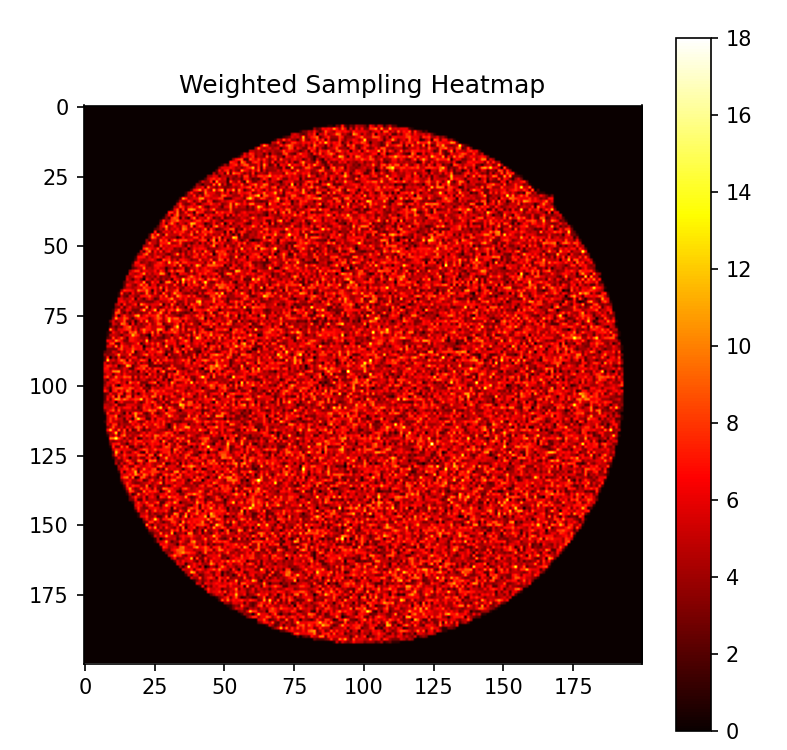
\includegraphics[width=\textwidth]{imaxes/muestraje/random_sampling_heatmap.png}
        \caption{Random sampling heatmap}
        \label{fig:random_sampling_heatmap}
    \end{subfigure}
    \hfill
    \begin{subfigure}[b]{0.3\textwidth}
        \centering
        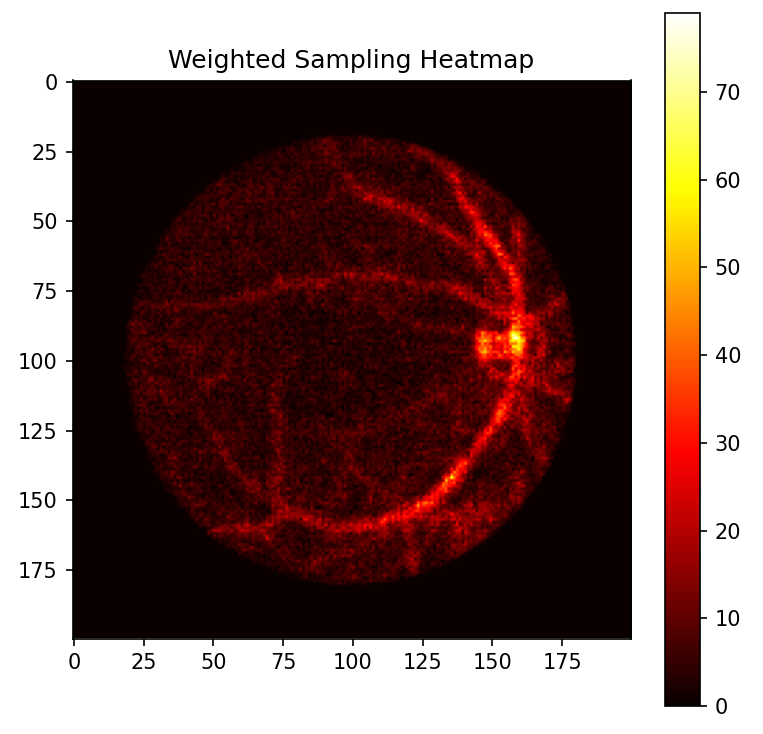
\includegraphics[width=\textwidth]{imaxes/muestraje/weighted_sampling_heatmap.png}
        \caption{Weighted sampling heatmap}
        \label{fig:weighted_sampling_heatmap}
    \end{subfigure}
    \hfill
    \begin{subfigure}[b]{0.3\textwidth}
        \centering
        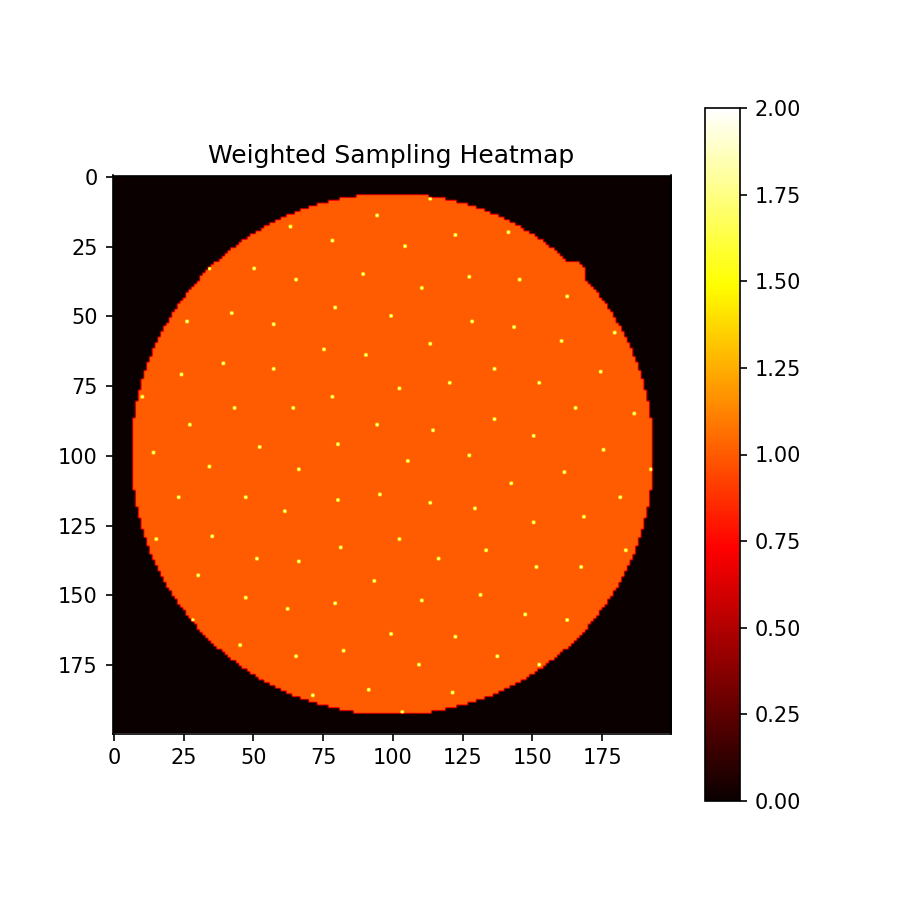
\includegraphics[width=\textwidth]{imaxes/muestraje/uniform_sampling_heatmap.png}
        \caption{Uniform sampling heatmap (100 points)}
        \label{fig:uniform_sampling_heatmap}
    \end{subfigure}
    \caption{Heatmaps illustrating the different sampling strategies implemented.}
    \label{fig:sampling_heatmaps}
\end{figure}

\subsubsection{Initialization Lottery}
\label{subsubsec:loteria_inicializacion}
Another methodology designed was the implementation of the initialization lottery. This technique consists of testing different random initializations of the network weights to determine which ones are most beneficial for convergence and final model performance, and selecting the best initialization to complete training

\subsubsection{Dynamic Batch Size Adjustment}
\label{subsubsec:axuste_dinamico_batch_size}
Dynamic batch size adjustment was implemented, which consists of increasing the number of samples taken by the network throughout training. To carry out this strategy, the epochs are divided into different phases, where each phase uses a different batch size, usually starting with smaller sizes and progressively increasing them.

\section{Evaluation Methods}
\label{sec:Métodos de Avaliación}

The evaluation of registration system performance constitutes a fundamental aspect to determine the effectiveness of the implemented modifications.
The evaluation process is divided into two complementary approaches: quantitative evaluation, which uses objective numerical metrics, and qualitative evaluation, which analyzes results visually to detect artifacts or unwanted deformations that may escape numerical metrics.

Both evaluations are necessary to obtain a complete view of registration quality, as quantitative evaluation may not be sufficient to detect visual problems that are not reflected in the metrics.

\subsection{Quantitative Evaluation}\label{subsec:Avaliación Cuantitativa}

We use as quantitative evaluation method the one proposed by FIRE \cite{FIRE}
generating a graph where the x-axis represents the error threshold value and the y-axis shows the percentage of image pairs that were successfully registered for each error threshold.

The registration error is calculated using the mean Euclidean distance between corresponding points in the fixed and moving images:

\begin{figure}[tbp]
    \centering
    \[
    E = \frac{1}{N} \sum_{i=1}^{N} \left\| p_i^{\text{fixo}} - T(p_i^{\text{móbil}}) \right\|
    \]
    \caption{Registration error calculation using Euclidean distance.}
    \label{fig:erro_registro}
\end{figure}

where N is the number of landmarks, p are the point coordinates and T is the applied transformation.

When the registration error between an image pair is below the threshold, the registration is considered successful and vice versa. This results in a monotonic and continuous curve that reflects the relationship between success rate and target precision, thus avoiding the need to establish an arbitrary threshold.
These graphs are used to illustrate registration accuracy both for individual cases (where the percentage of successfully registered point pairs is used)
and for the complete dataset.
This metric facilitates comparison between different competing methods and allows selecting the most suitable one according to the desired precision.

Additionally, in FIRE the evaluation will be segmented into 3 image categories (S, P and A) to analyze registration performance in each of them, since each category presents different challenges and characteristics.

While FIRE already provides the landmarks for evaluation, RFMID does not.
Therefore, for RFMID, we use the same evaluation method, but generating the points manually so that they cover the interior of the fixed image mask (separated by 50 pixels from each other).

\begin{figure}[tbp]
    \centering
    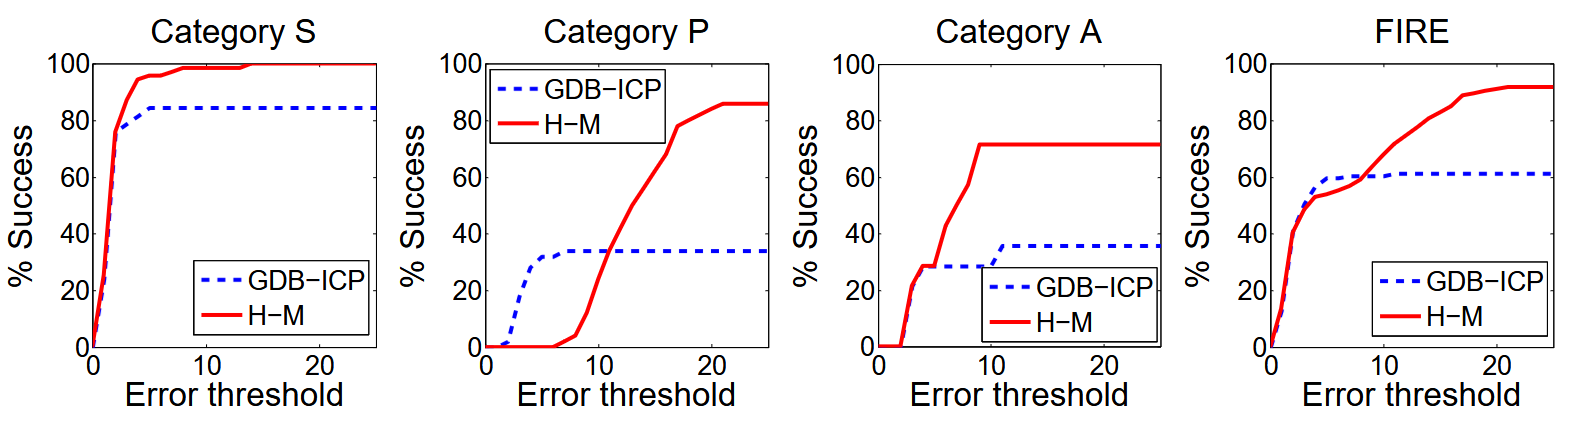
\includegraphics[width=0.8\textwidth]{imaxes/fire_aval.png}
    \caption{FIRE evaluation graph \cite{FIRE}}
    \label{fig:fire_aval}
\end{figure}

In the case of RFMiD, we will divide the dataset into several categories depending on the registration difficulty, which is calculated using the Frobenius norm of a matrix $A \in \mathbb{R}^{m \times n}$.
This is a generalization of the Euclidean distance applied to matrices, where images with larger transformations are considered more difficult.

\begin{figure}[tbp]
    \centering
    \[
    \|A\|_F = \sqrt{\sum_{i=1}^{m} \sum_{j=1}^{n} |a_{ij}|^2}
    \]
    \caption{Frobenius norm of a matrix $A \in \mathbb{R}^{m \times n}$, where $a_{ij}$ are the elements of matrix $A$.}
    \label{fig:frobenius_norm}
\end{figure}

In some cases we will also use the mean distance between corresponding points as a complementary metric to evaluate registration quality, since the success rate may not be sufficient to detect changes.

\subsection{Qualitative Evaluation}
\label{subsec:Avaliación Cualitativa}

In the case of this work, qualitative evaluation becomes very important, since quantitative evaluation only compares a reduced number of points in each image pair.
Visual evaluation allows detecting problems that are not reflected in quantitative metrics, such as visual artifacts or unwanted deformations,
especially in registrations that have local deformations that may not coincide with any point.

In the case of the FIRE dataset \cite{FIRE}, visual evaluation is especially relevant, since only 10 reference points per image are provided, which may not be sufficient to evaluate registration quality in many areas of the image.
Since in RFMID \cite{RFMiD} manually generated reference points are used that cover the entire image, visual evaluation is somewhat less relevant, since it is more likely that an incorrect local deformation will be detected by some point and be reflected in the metrics.

In order to easily identify different visual artifacts or unrealistic transformation, different tools are used such as image composition, displacement vector visualization and comparison of images before and after registration.
Figure \ref{fig:visex} shows some examples of these.

\begin{figure}[tbp]
    \centering
    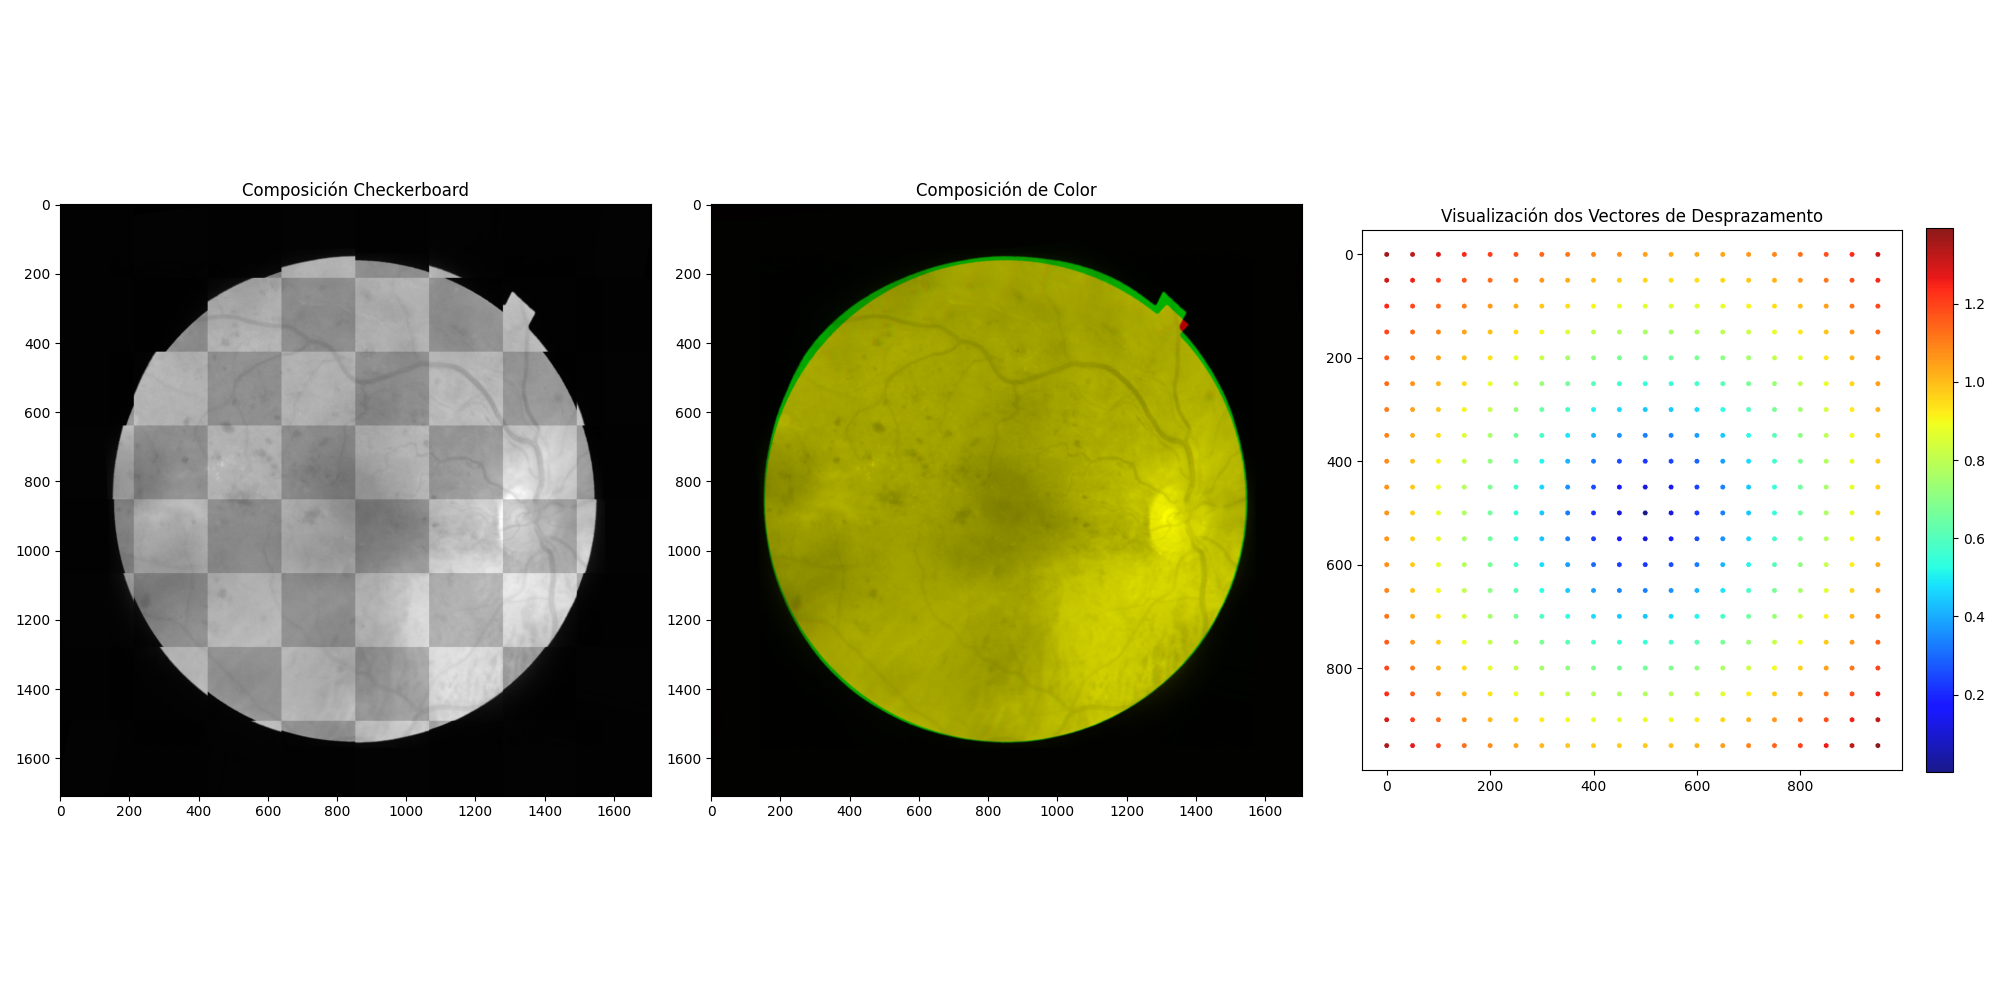
\includegraphics[width=0.9\textwidth]{imaxes/visex.png}
    \caption{Examples of visual evaluation: (a) Checkerboard image composition, (b) Color image composition, (c) Displacement vector visualization.}
    \label{fig:visex}
\end{figure}